\chapter{Counting}\label{chapter:combinatorial-methods}

Combinatorics, or discrete mathematics, is mathematics of finite structures. A central theme in combinatorics is counting, establishing a closed form for the number of objects of a certain kind. Sometimes, counting methods can be used to obtain results in number theory. In this lecture we will use a combinatorial argument to show that the product
\begin{equation*}
  n(n+1)\cdots(n+k-1)
\end{equation*}
of any $k$ consecutive natural numbers is always divisible by $k!$. We will also establish the binomial theorem, which has a myriad of applications throughout mathematics.

\section{The Standard Finite Sets}

\begin{definition}
  The \emph{standard finite set} $[n]$ with $n$ elements is defined by
  \begin{equation*}
    [n]:=\{0,\ldots,n-1\}=\{x\in\mathbb{N}\mid x<n\}.
  \end{equation*}
\end{definition}

We now turn to the question of formally defining the process of counting. What does it mean when we say that a set $X$ has $n$ elements? It means that we can, at least in principle, label each element of $X$ with a number $0\leq i<n$ in such a way that every number $0\leq i<n$ is used at least once, and that no two elements of $X$ got assigned the same number.

\begin{definition}
  A function $f:X\to Y$ is said to be a \emph{bijection} if for every $y\in Y$, the set
  \begin{equation*}
    \{x\in X\mid f(x)=y\}
  \end{equation*}
  consisting of all elements $x\in X$ with value $f(x)=y$ has exactly one element. Some authors call bijections \emph{one-to-one correspondences}.
\end{definition}

\begin{definition}
  A function $f:X\to Y$ is said to be \emph{invertible} if there is a function $g:Y\to X$ such that
  \begin{equation*}
    f(g(y))=y \qquad\text{and}\qquad g(f(x))=x
  \end{equation*}
  for every $x\in X$ and $y\in Y$.
\end{definition}

\begin{theorem}
  A function $f:X\to Y$ is a bijection if and only if it is invertible.
\end{theorem}

\begin{proof}
  Suppose first that $f$ is a bijection. To construct its inverse $g$, we must assign to each element $y\in Y$ an element $x\in X$. By the assumption that $f$ is a bijection, we are given that the set
  \begin{equation*}
    \{x\in X\mid f(x)=y\}
  \end{equation*}
  has exactly one element. Thus, we let $g(y)$ be the unique element of this set. By definition, we have $f(g(y))=y$. To see that $g(f(x))=x$, note that $x$ is the unique element in the set
  \begin{equation*}
    \{x'\in X\mid f(x')=f(x)\}.
  \end{equation*}
  Thus, if we can show that $g(f(x))$ is also in this set, then it follows that $g(f(x))=x$. In other words, our plan is to show that $f(g(f(x)))=f(x)$. However, this follows at once from the definition of $g$, using the element $y:=f(x)$. This shows that $f$ is invertible.

  For the converse, assume that $f$ is invertible with inverse $g$, and consider the set
  \begin{equation*}
    \{x\in X\mid f(x)=y\}.
  \end{equation*}
  Observe that $g(y)$ is in this set, since $f(g(y))=y$ by the assumption that $g$ is an inverse of $f$. Thus, the set has at least one element. It remains to show that it has at most one element. To see this, consider two elements $x$ and $x'$ such that $f(x)=y$ and $f(x')=y$. Then we obtain that
  \begin{equation*}
    x=g(f(x))=g(y)=g(f(x'))=x'.
  \end{equation*}
  This shows that any two elements in the set $\{x\in X\mid f(x)=y\}$ must be equal, so it has at most one element.
\end{proof}

\section{Counting Bijections}

\begin{definition}
  A function $f:A \to B$ is said to be a \emph{bijection} if for every $y\in B$, the \emph{preimage} of $b$
\begin{equation*}
  f^{-1}(y) := \{x\in A\mid f(x)=y\}
\end{equation*}
has exactly one element. We write $A\cong B$ for the set of bijections from $A$ to $B$.
\end{definition}

A function $f:A \to B$ is a bijection precisely when it is \emph{invertible} in the sense that there is a function $g:B\to A$ such that $f\circ g=\mathrm{id}_B$ and $g\circ f=\mathrm{id}_A$. Here, the composite $g\circ f$ of $g$ and $f$ is the function $x\mapsto g(f(x))$ defined by applying $g$ to the value $f(x)$ of $f$ at the input variable $x$.

The \define{factorial function} $n\mapsto n!$ is defined recursively by
  \begin{align*}
    0! & := 1 \\
    (n+1)! & := n!(n+1).
  \end{align*}
  In the following proposition we prove the number of bijections $[n]\cong[n]$ on the \emph{standard $n$-element set}
  \begin{equation*}
    [n] := \{0,\ldots,n-1\}.
  \end{equation*}
  is the number $n!$. In other words, the factorial function counts the number of bijections on the standard $n$-element set.
  
\begin{proposition}
  The number of bijections $[n]\cong [n]$ from the standard $n$-element set to itself is exactly $n!$.
\end{proposition}

\begin{proof}
  The proof is by induction on $n$. For the base case, let $n=0$. Then $[n]$ is an empty set, and there is exactly one function $[n]\to [n]$, the empty function. This function is a bijection, because assuming an element of an empty set is an inherent contradiction.

  Now suppose that the number of bijections $[n]\cong[n]$ is $n!$. We claim that for each $y\in[n+1]$ there are exactly $n!$ bijections $f:[n+1]\cong[n+1]$ such that $f(n)=y$.

  To see this, we first define the \emph{transposition function} $s_{y,n}$ defined by
  \begin{equation*}
    s_{y,n}(x) =
    \begin{cases}
      n & \text{if }x=y, \\
      y & \text{if }x=n, \\
      x & \text{otherwise.}
    \end{cases}
  \end{equation*}
  In other words, the function $s_{y,n}$ swaps the elements $n$ and $y$, and leaves the other elements fixed. This function is a bijection, because we can verify that the preimage $s_{y,n}^{-1}(z)$ is a singleton set for every $z\in[n+1]$. The preimage $s_{y,n}^{-1}(n)$ is the singleton set $\{y\}$; the preimage $s_{y,n}^{-1}(y)$ is the singleton set $\{n\}$, and the preimage $s_{y,n}^{-1}(x)$ is the singleton set $\{x\}$ otherwise.

  Now we observe that the function
  \begin{equation*}
    ([n+1]\cong[n+1])\to ([n+1]\cong[n+1])
  \end{equation*}
  given by $g\mapsto s\circ g$ is itself a bijection, because it is an invertible function. Indeed, it is its own inverse, because $s\circ s\circ g = g$ for any bijection $g$.

  Thus, if $f:[n+1]\cong[n+1]$ is a bijection such that $f(n)=y$, then $s\circ f$ is a bijection satisfying $s(f(n))=n$. In other words, every bijection satisfying $f(n)=y$ corresponds uniquely to a bijection satisfying $f(n)=n$.

  Now we observe that there are exactly $n!$ bijections $f:[n+1]\cong[n+1]$ satisfying $f(n)=n$. Indeed, such bijections are uniquely determined by their restriction to the set $[n]$, and by the induction hypothesis there are $n!$ such bijections. Since there are $n+1$ possible choices of a value $y$, we conclude that there are $n!(n+1)$ bijections altogether from $[n+1]$ to $[n+1]$.
\end{proof}

To wrap up this section, we give a lower bound for the factorial $n!$. Recall that the exponential function is defined by the infinite series
\begin{equation*}
  e^x := \sum_{n=0}^\infty \frac{x^n}{n!}.
\end{equation*}
Here, the quantity $e:=\sum_{n=0}^\infty \frac{1}{n!}$ is Euler's number, of which the first few terms are
\begin{equation*}
  \frac{1}{0!}+\frac{1}{1!}+\frac{1}{2!}+\frac{1}{3!}+\frac{1}{4!}+\frac{1}{5!} + \cdots = 1+1+\frac{1}{2}+\frac{1}{6}+\frac{1}{24}+\frac{1}{120}+\cdots.
\end{equation*}
The terms from $1/0!$ to $1/5!$ add up to $2+\frac{86}{120}\approx 2.71\cdots$, which correctly estimates the value of $e$ up to two decimal digits.

\begin{theorem}\label{theorem:elementary-estimate-factorial}
  For any positive natural number $n$, we have the strict inequality
  \begin{equation*}
    \left(\frac{n}{e}\right)^n<n!.
  \end{equation*}
\end{theorem}

\begin{proof}
  For positive $x$, every term $\frac{x^n}{n!}$ contributes a positive amount to the exponential function. This gives the strict inequality
  \begin{equation*}
    \frac{x^n}{n!}<e^x.
  \end{equation*}
  We may simply take $x=n$ to obtain
  \begin{equation*}
    \frac{n^n}{n!}<e^n,
  \end{equation*}
  and the theorem is obtained by rearranging.
\end{proof}

\begin{remark}
  The strict lower bound for $n!$ given in \cref{theorem:elementary-estimate-factorial} is not the best known estimate of the factorial function. Nevertheless, its proof is elementary, and it can be used in basic number-theoretic estimates. The best approximation to the factorial function is given by Stirling's approximation formula:
  \begin{equation*}
    n!\sim \sqrt{2\pi n}\left(\frac{n}{e}\right)^n.
  \end{equation*}
  This means that the ratio of the quantities $n!$ and $\sqrt{2\pi n}(n/e)^n$ tends to $1$ as $n$ becomes arbitrarily large. While Stirling's approximation formula is certainly applicable in number theory, we shall have no need for it in the present introduction to the subject and therefore we will omit the proof.
\end{remark}

\section{Counting Subsets}

A subset $A$ of a set $X$ is a set consisting entirely of elements of $X$. Subsets may be empty or they may contain all elements of $X$. When $A$ is a subset of $X$, we write
\begin{equation*}
  A\subseteq X.
\end{equation*}
Subsets of $X$ can be formed using predicates over the elements of $X$. Predicates are propositions or conditions about indeterminate elements. For example, the predicate that $n$ is an even natural number is a predicate with the indeterminate natural number $n$. This predicate determines the subset of all even natural numbers
\begin{equation*}
  0,2,4,6,\ldots.
\end{equation*}
Often, we write $P(x)$ for a predicate on the indeterminate element $x$. The subset determined by this predicate is the set of all the elements $x$ that satisfy the condition $P(x)$. Such sets are conveniently defined by \emph{set-builder notation}:
\begin{equation*}
  \{x\in X\mid P(x)\}.
\end{equation*}
For example, the set of even natural numbers can be written in set-builder notation as follows:
\begin{equation*}
  \{n\in\mathbb{N}\mid \text{$n$ is even}\}.
\end{equation*}
Here, the condition that $n$ is even could also be expressed through the logical formula
\begin{equation*}
  \exists_{(k\in\mathbb{N})}2k=n
\end{equation*}
asserting that there exists a natural number $k$ such that the number $2k$ is equal to the number $n$. Nevertheless, we often find ourself preferring expressions in natural language that convey the intended meaning more easily.

To avoid any complications of constructive logic, we shall assume that all predicates are decidable, meaning that for every predicate $P(x)$ on the indeterminate element $x$ and for any element $a$, we can decide whether or not the property $P(a)$ holds. The typical predicates of concern in elementary number theory, until the real and complex numbers are considered, are indeed decidable.

Subsets of a finite set $X$ are determined by a function $X\to \{0,1\}$. Indeed, given a subset $A$ of $X$, we define its \emph{characteristic function} $\chi_A$ by
\begin{equation*}
  \chi_A(x):=
  \begin{cases}
    1 & \text{if $x\in A$}, \\
    0 & \text{otherwise}.
  \end{cases}
\end{equation*}
Conversely, any function $f:X\to \{0,1\}$ determines the subset
\begin{equation*}
  \{x\in X\mid f(x)=1\}.
\end{equation*}
Thus, we can go back and forth between (1) subsets of a set, (2) predicates on a set, and (3) functions from a set into $\{0,1\}$. All of these are equivalent descriptions of the concept of subset.

Since subsets of $X$ are equivalently described as functions from $X$ into the set $\{0,1\}$, it follows immediately that if $X$ is an $n$-element set, then the number of subsets of $X$ is $2^n$. To put it another way: In order to determine a subset of $X$, there are two possibilities for every element of $X$. It is either in the subset, or it isn't. Thus, there are $2^n$ combined possibilities determining distinct subsets.

Knowing that the total number of subsets of an $n$-element set is $2^n$, we now turn to the question: How many $k$-element subsets are there of an $n$-element set? For example, the six $2$-element subsets of the set $\{1,2,3,4\}$ are
\begin{equation*}
  \{1,2\},~\{1,3\},~\{1,4\},~\{2,3\},~\{2,4\},~\text{and}~\{3,4\}.
\end{equation*}
The binomial coefficients are introduced precisely to answer this question for generela $n$ and $k$.

\begin{definition}
  The \emph{binomial coefficients} \(\binom{n}{k}\) are defined recursively by
  \begin{align*}
    \binom{0}{0} & := 1 & \binom{0}{k+1} & := 0 \\
    \binom{n+1}{0} & := 1 & \binom{n+1}{k+1} & := \binom{n}{k} + \binom{n}{k+1}.
  \end{align*}
\end{definition}

The binomial coefficients can be arranged in \emph{Pascal's triangle}, where each entry is the sum of the two directly above it. At the top of the triangle we find the binomial coefficient $\binom{0}{0}$. This is $0$th row of Pascal's triangle. In the $n$th row from the top, we find the binomial coefficients $\binom{n}{k}$ for $0\leq k\leq n$.

\begin{figure}[t]
  \centering
  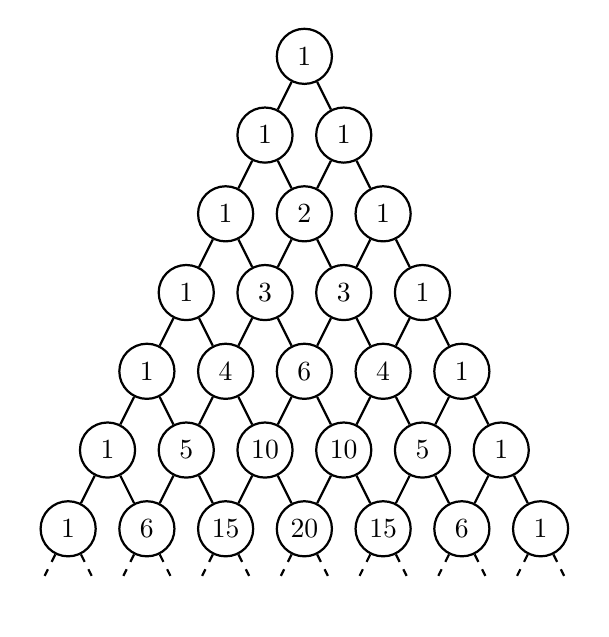
\begin{tikzpicture}[every node/.style={
      draw,
      thick,
      circle,
      minimum size=7mm,
      inner sep=1pt,
      align=center
    }]
    % nodes
    \foreach \n in {0,...,6}{
      \foreach \r in {0,...,\n}{
        \pgfmathtruncatemacro{\val}{int(factorial(\n)/(factorial(\r)*factorial(\n-\r)))}
        \node (n\n\r) at (\r-\n/2,-\n) {\val};
      }
    }
    % normal connections
    \foreach \n in {0,...,5}{
      \pgfmathtruncatemacro{\nn}{\n+1}
      \foreach \r in {0,...,\n}{
        \pgfmathtruncatemacro{\rp}{\r+1}
        \draw[thick] (n\n\r) -- (n\nn\r) (n\n\r) -- (n\nn\rp);
      }
    }
    % bottom‐row extensions (solid then dotted)
    \foreach \r in {0,...,6}{
      % down‐left
      %\draw[thick,solid, shorten >=6mm]  (n6\r) -- ++(-0.5cm,-1cm);
      \draw[thick,dashed,shorten >=4.5mm]   (n6\r) -- ++(-0.5cm,-1cm);
      % down‐right
      % \draw[thick,solid, shorten >=6mm]  (n6\r) -- ++( 0.5cm,-1cm);
      \draw[thick,dashed,shorten >=4.5mm]   (n6\r) -- ++( 0.5cm,-1cm);
    }
  \end{tikzpicture}
  \caption[Pascal's triangle]{\label{figure:pascals-triangle}Pascal's triangle.}
\end{figure}

\begin{theorem}
  Consider an \(n\)-element set \(S\), and a natural number \(k\). Then the number of \(k\)-element subsets of \(S\) is the binomial coefficient \(\binom{n}{k}\).
\end{theorem}

\begin{proof}
  Since the binomial coefficients are defined recursively, this theorem is best proven by induction on both variables.

  If \(S\) has no elements and \(k=0\), then there is exactly one subset of \(S\) having \(k\) elements, the empty subset. This shows that the number of \(0\)-element subsets of \(S\) is \(\binom{0}{0}\).

  If \(S\) has no elements, then there are no \((k+1)\)-element subsets of \(S\), since any \((k+1)\)-element subset has at least one element, but \(S\) has no elements. This shows that the number of \((k+1)\)-element subsets of \(S\) is \(\binom{0}{k+1}\).

  If \(S\) has \(n+1\) elements, then there is exactly one subset of \(S\) with no elements, the empty subset. This shows that the number of \(0\)-element subsets of \(S\) is \(\binom{n+1}{0}\).

  If \(S\) has \(n+1\) elements, then \(S\) has at least one element \(x_0\). Now there are two classes of subsets having \((k+1)\) elements: the subsets containing \(x_0\) and the subsets not containing \(x_0\). A \((k+1)\)-element subset of \(S\) containing \(x_0\) is equivalently described as a \(k\)-element subset of the \(n\)-element set \(S\setminus\{x_0\}\), because its \((k+1)\)st element is the element \(x_0\). By the induction hypothesis, there are exactly \(\binom{n}{k}\) such subsets. Furthermore, a \((k+1)\)-element subset of \(S\) not containing \(x_0\) is equivalently described as a \((k+1)\)-element subset of the \(n\)-element set \(S\setminus\{x_0\}\). By the induction hypothesis, there are exactly \(\binom{n}{k+1}\) such subsets. Combining these two observations, we find that the number of \((k+1)\)-element subsets of \(S\) is
  \begin{equation*}
    \binom{n}{k+1} + \binom{n}{k} = \binom{n+1}{k+1}.\qedhere
  \end{equation*}
\end{proof}

\begin{definition}
  We define the set $P_S(k)$ of $k$-permutations of a set $S$ recursively by:
  \begin{enumerate}
  \item The set $P_S(0)$ of $0$-permutations of $S$ is the set $\{\ast\}$ with one element.
  \item The set $P_S(k+1)$ of $(k+1)$-permutations of $S$ is the set
    \begin{equation*}
      \{(s,t) \mid s\in S,\ t\in P_{S\setminus\{s\}}(r)\}
    \end{equation*}
    of pairs $(s,t)$ consisting of an element in $S$ and an $k$-permutation of the set $S\setminus\{s\}$.
  \end{enumerate}
\end{definition}

\begin{lemma}
  The number of $k$-permutations of an $n$-element set $S$ is the number $\rpermutation{n}{k}$ defined by
  \begin{equation*}
    \rpermutation{n}{k} := n(n-1)\cdots(n-k+1).
  \end{equation*}
\end{lemma}

\begin{proof}
  The proof is by induction on $k$. There is exactly one $0$-permutation of any $n$-element set. To see that the number of $(k+1)$-permutations of an $n$-element set is $n\cdots(n-k)$, note that such a $(k+1)$-permutation consists of a choice of an element of $S$, and a $k$-permutation on the remaining $n-1$-element set of elements. Thus, the number of $(k+1)$-permutations on an $n$-element set is $n$ times the number of $k$-permutations on an $(n-1)$-element set, i.e., it is
  \begin{equation*}
    n(n-1)\cdots((n-1)-k+1)=n(n-1)\cdots(n-k).\qedhere
  \end{equation*}
\end{proof}

\begin{proposition}\label{proposition:characterize-k-permutations}
  There is a bijection between the set of $k$-permutations of an $n$-element set $S$, and the set
  \begin{equation*}
    \{(A,f) \mid A\subseteq S, f : \{0,\ldots,k-1\}\cong A\}
  \end{equation*}
  of pairs $(A,f)$ consisting of a subset $A\subseteq S$ and a bijection $\{0,\ldots,k-1\}\cong A$.
\end{proposition}

\begin{proof}
  There is exactly one $0$-permutation of any $n$-element set $S$, and likewise the set of empty subsets $A$ of $S$ equipped with a bijection $[0]\cong A$ also contains exactly one element: the empty subset equipped with the empty bijection.

  For the inductive step, consider a $(k+1)$-permutation $(s,t)$ of $S$, consisting of an element $s$ and a $k$-permutation $t$ of the set $S\setminus\{s\}$. By the induction hypothesis, the $k$-permutation $t$ corresponds uniquely to a subset $A\subseteq S\setminus\{s\}$ equipped with a bijection $f:[n]\cong A$. Thus, the $(k+1)$-permutation $(s,t)$ corresponds to the subset $B:=A\cup\{s\}\subseteq S$, equipped with the bijection $g:[n+1]\cong B$ given by $g(x):=f(x)$ for $x<n$ and $g(n):= s$.
\end{proof}

\begin{proposition}
  The product $n(n-1)\cdots(n-k+1)$ of any $k$ consecutive numbers is divisible by $k!$.
\end{proposition}

\begin{proof}
  By \cref{proposition:characterize-k-permutations} there is a bijection between the set of $k$-permutations of the set $S:=[n]$, and the set
  \begin{equation*}
    \{(A,f) \mid A\subseteq S, f : \{0,\ldots,k-1\}\cong A\}.
  \end{equation*}
  These two sets therefore have the same number of elements. Thus, it follows that
  \begin{equation*}
    n(n-1)\cdots(n-k+1) = \binom{n}{k}\cdot k!,
  \end{equation*}
  showing that the left-hand side is divisible by $k!$.
\end{proof}

\begin{corollary}
  \emph{Formula for binomial coefficients.} For any two natural numbers $n$ and $k$, we have
  \begin{equation*}
    \binom{n}{k}=\frac{n!}{k!(n-k)!}.
  \end{equation*}
\end{corollary}

\begin{proof}
  By the previous proposition we have $\binom{n}{k}\cdot k!= \rpermutation{n}{k}= n!/k!$.
\end{proof}

\section{The Binomial Theorem}

If we expand the exponent $(x+y)^3$, we get
\begin{align*}
  (x+y)^3  & = (x+y)^2(x+y) \\
           & = (x^2 + 2xy + y^2)(x+y) \\
           & = x^3 + 2x^2y + xy^2 + x^2y + 2xy^2 + y^3 \\
           & = x^3 + 3x^2y + 3xy^2 + y^3.
\intertext{Going further, if we expand the exponent $(x+y)^4$, we get}
  (x+y)^4 & = (x^3 + 3x^2y + 3xy^2 + y^3)(x + y) \\
          & = x^4 + 3x^3y + 3x^2y^2 + xy^3 + x^3y + 3x^2y^2 + 3xy^3 + y^4 \\
          & = x^4 + 4x^3y + 6x^2y^2 + 4xy^3 + y^4.
\end{align*}

Now we might recognize an emerging pattern in the coefficients of these polynomials: they are all binomial coefficients! The binomial theorem generalizes this result for all exponents $n$.

The binomial theorem has many proofs, including combinatorial proofs and algebraic proofs. All these proofs have their own merits. We will present here an algebraic proof, using induction, since it is the most easily applicable to settings other than the integers.

\begin{theorem}\label{theorem:binomial-theorem}
  \emph{The binomial theorem.} In any number system, such as the natural numbers, the integers, the rational numbers, the reals, the complex numbers\footnote{More generally, the binomial theorem applies to any semiring, conditional on the assumption that $xy=yx$.}, we have
  \begin{equation*}
    (x+y)^n = \sum_{k=0}^n \binom{n}{k}x^ky^{n-k}.
  \end{equation*}
\end{theorem}

\begin{proof}
  We prove the statement by induction on $n$. In the base case, we find that both sides of the equation
  \begin{equation*}
    (x+y)^0=\sum_{k=0}^0 \binom{n}{k}x^ky^{0-k}
  \end{equation*}
  evaluate to $1$, so the equation is true. In the inductive step, we have that
  \begin{align*}
    (x+y)^{n+1} & =(x+y)\sum_{k=0}^n \binom{n}{k}x^ky^{n-k} \\
                & = \sum_{k=0}^n \binom{n}{k}x^{k+1}y^{n-k} + \sum_{k=0}^n\binom{n}{k}x^ky^{n-k+1} \\
                & = x^{n+1} + \sum_{k=0}^{n-1} \binom{n}{k}x^{k+1}y^{n-k} + \sum_{k=1}^n\binom{n}{k}x^ky^{n-k+1} + y^{n+1} \\
                & = x^{n+1} + \sum_{k=1}^{n} \binom{n}{k-1}x^{k}y^{n-k+1} + \sum_{k=1}^n\binom{n}{k}x^ky^{n-k+1} + y^{n+1} \\
                & = x^{n+1} + \sum_{k=1}^n \left(\binom{n}{k-1}+\binom{n}{k}\right)x^ky^{n-k+1}+y^{n+1} \\
    & = \sum_{k=0}^{n+1} \binom{n+1}{k}x^ky^{(n+1)-k}.\qedhere
  \end{align*}
\end{proof}

The binomial theorem has a long history. The earliest known references to aspects of the binomial theorem are found in the Chinese mathematical text \emph{Jiuzhang Suanshu} (Nine Chapters on the Mathematical Art), from approximately the 2nd century BCE. Around the 11th century CE, the Chinese mathematician Jia Xian described a method for calculating binomial coefficients, which corresponds to what we now refer to as Pascal’s triangle. This method was popularized by Yang Hui in the 13th century CE, and thus Pascal’s triangle is sometimes called the \emph{Yang Hui triangle} in China. Isaac Newton was the first to generalize the binomial theorem to non-integer number systems, in 1687 in his \emph{Principia Mathematica}.

\section{The Inclusion-Exclusion Principle}

Consider two subsets $A$ and $B$ of a set $X$. The \emph{union} of $A$ and $B$ is the set
\begin{equation*}
  A\cup B :=\{x\in X\mid x\in A\text{ or }x\in B\}.
\end{equation*}
Given that $X$ is a finite set, we may wish to determine the number of elements in $A\cup B$. Note, however, that in general the answer is not found by simply adding up the number of elements of $A$ and the number of elements in $B$. Indeed, some elements might be contained in both subsets, and they would therefore be counted double. Since every element in the intersection $A\cap B$ is counted twice, the correct formula for the number of elements in $A\cup B$ is:
\begin{equation*}
  |A\cup B| = |A| + |B| - |A\cap B|.
\end{equation*}

\begin{example}
  Consider the set $X=\{1,\ldots,100\}$, and our goal is to find the number of integers in $X$ that are neither divisible by $2$ nor by $3$. This problem can be solved with the inclusion-exclusion principle.

  Let $A$ and $B$ be the subsets of $X$ consisting of numbers divisible by $2$ and by $3$, respectively. The set $A\cap B$ then consists of all the numbers divisible by both $2$ and $3$; that is, the numbers divisible by $6$.

  There are $50$ numbers in $X$ divisible by $2$, there are $33$ numbers in $X$ divisible by $3$, and there are $16$ numbers in $X$ divisible by $6$. Thus, the total count of numbers in $X$ not divisible by either $2$ or $3$ is
  \begin{equation*}
    100-50-33+16=33.
  \end{equation*}
\end{example}

The inclusion-exclusion principle is a generalization of the formula for the number of elements of $A\cup B$ to any finite number of subsets of a set $X$. To see the pattern, let us consider the case with three subsets $A$, $B$, and $C$ of a set $X$. Now, if we wish to determine the number of elements in $A\cup B\cup C$, we can again start by adding the numbers $|A|$, $|B|$, and $|C|$. Every element that was in exactly one of the three subsets is correctly accounted for, but we have overcounted the elements in $A\cap B$, $A\cap C$, and $B\cap C$. If we subtract the numbers $|A\cap B|$, $|A\cap C|$, and $|B\cap C|$ from our total, then we have correctly accounted for every element that was in at most two subsets. However, now we have subtracted every element in $A\cap B\cap C$ three times from our count, so we must add them again to arrive at the correct number:
\begin{equation*}
  |A\cup B\cup C|=|A|+|B|+|C|-|A\cap B|-|A\cap C|-|B\cap C|+|A\cap B \cap C|.
\end{equation*}
Thus, we see an alternating pattern emerging: Single sets are added, intersections of two sets are subtracted, triple intersections are added again, and so on. The inclusion-exclusion principle is stated with this alternating pattern.

\begin{theorem}\label{theorem:inclusion-exclusion-principle}
  Consider a set $X$ and a finite family of subsets $A_i\subset X$ indexed by $1\leq i\leq n$. Then the number of elements in the union of the subsets $A_i$ is given by
  \begin{equation*}
    |A_1\cup\cdots\cup A_n|=\sum_{k=1}^n (-1)^{k+1}\left(\sum_{1\leq i_1<\cdots<i_k\leq n}|A_{i_1}\cap\cdots\cap A_{i_k}|\right).
  \end{equation*}
\end{theorem}

\begin{exercises}
  \exercise Prove that $2^n<n!$ for all $n\geq 4$.
  \exercise Prove that
  \begin{equation*}
    \sum_{k=0}^n \binom{n}{k} = 2^n
  \end{equation*}
  in three different ways: using the binomial theorem, by a direct proof by induction, and by a combinatorial proof.
  \exercise
  \begin{enumerate}
  \item Show that in each row of Pascal's triangle, the number of odd entries is always a power of $2$.
  \item Show that in the $n$th row of Pascal's triangle all the entries are odd precisely when $n=2^k-1$ for some $k$.
  \end{enumerate}
  \exercise Prove that
  \begin{equation*}
    \sum_{k=0}^n\binom{n}{k}(-1)^k = 0.
  \end{equation*}
  Conclude that
  \begin{equation*}
    \sum_{k=0}^{\lfloor n/2\rfloor}\binom{n}{2k} =\sum_{k=0}^{\lfloor (n-1)/2\rfloor}\binom{n}{2k+1}.
  \end{equation*}
  In this formula, the floor $\lfloor x\rfloor$ of a number $x$ is the largest integer below or equal to $x$.
  \exercise \label{exercise:hockey-stick-identity}\emph{The hockey-stick identity.} Show that
  \begin{equation*}
    \sum_{i=k}^m\binom{i}{k}=\binom{m+1}{k+1}.
  \end{equation*}
  \exercise \emph{The Chu--Vandermonde identity.} Use the binomial theorem at the polynomial $(x+1)^m(x+1)^n$ to show that
  \begin{equation*}
    \sum_{i=0}^k \binom{m}{i}\binom{n}{k-i} = \binom{m+n}{k}.
  \end{equation*}
  \exercise Show that
  \begin{equation*}
    \sum_{k=0}^n \binom{n}{k}^2 = \binom{2n}{n}.
  \end{equation*}
  The binomial coefficient $\binom{2n}{n}$ is also called the \emph{central binomial coefficient}.
  \exercise \label{exercise:estimates-central-binomial-coefficients}Show that the strict inequalities
  \begin{equation*}
    \frac{4^n}{2n+1} < \binom{2n}{n} < 4^n
  \end{equation*}
  hold for all $n\geq 1$.
  \exercise Show that
  \begin{equation*}
    \sum_{k=0}^n\prod_{i=0}^m (k+i) = (m+1)!\binom{n+m+1}{m+2}.
  \end{equation*}
  \exercise Find the first $20$ positive integers that are not divisible by any Fibonacci number other than $1$. This is https://oeis.org/A147956
  \exercise Define the \emph{inclusion-exclusion sequence} $a_n$ by $a_0:=0$, $a_1:=1$, and let $a_{n+1}$ be the largest positive integer so that the number of positive integers $1\leq x < a_{n+1}$ not divisible by any $a_i$ for $2\leq i\leq n$ is $a_n$. Determine the values for $a_n$ for $1\leq n\leq 10$.
  \exercise Find a parametrization of all pairs $(m,n)$ of natural numbers such that $n^2-m^2$ is a number of the form $2^k$, and prove that your parametrization is a bijection.
  % \exercise
  % \begin{subexenum}
  % \item Find the first $20$ positive integers that are not divisible by any Fibonacci number other than $1$. %This is https://oeis.org/A147956
  % \item Determine for each $n$ the number of integers from $1$ to the $n$th Fibonacci number $F_n$ that are not divisible by any Fibonacci number other than $1$.
  % \end{subexenum}
  % \exercise The Pell numbers $P_n$ are defined by
  % \begin{equation*}
  %   P_0:=0,\qquad P_1:= 1,\qquad\text{and}\qquad P_{n+2}:=2P_{n+1}+P_n.
  % \end{equation*}
  % \begin{subexenum}
  % \item Find the first $20$ positive integers that are not divisible by any Pell number other than $1$.
  % \item Determine for each $n$ the number of integers from $1$ to the $n$th Pell number $P_n$ that are not divisible by any Pell number other than $1$.
  % \end{subexenum}
\end{exercises}

%%% Local Variables:
%%% mode: latex
%%% TeX-master: "elementary-number-theory"
%%% End:
